%% CHAPTER 2 (probably)
%% MODELLING and DATA

\chapter{Modelling and Data} %with GEOS-Chem} % Main chapter title
\label{Model} %better reference name?
  
\section{Introduction}
  %Why use models?
  % Models
  Models of ozone in the atmosphere are used broadly for international assessments of ozone related emissions \citep{Young2018}.
  \cite{Young2018} summarise current global ozone modelling standards and the metrics and processes used to evaluate these models.
  They show how models can be used to improve measurements, estimate concentrations in regions not sampled, and allow analysis of other processes which involve ozone (such as radiation).




\section{List of runs and outputs used in my work TODO: good place for this?}
  TODO: Go through work process and clarify these items
  \subsection{GEOS-Chem}
    \begin{enumerate}
      \item UCX 
      \begin{enumerate}
        \item Satellite output (1300-1400LT)
        \item Create shape factors for AMF recalculation in OMI
      \end{enumerate}
      
      \item Tropchem (standard)
      \begin{enumerate}
        \item satellite output, daily tracer averages
        \item Recreate the AMFs for OMI when running code from Dr. Paul Palmer, modified by Dr. Luke Surl.
        \item Combined with an identical run where isoprene emissions are halved in order to determine smearing.
        \item TODO: Compare total yearly isoprene emissions before and after new estimate.
      \end{enumerate}
    
      \item Tropchem(isoprene emissions halved)
      \begin{enumerate}
        \item Satellite output used to determine smearing.
      \end{enumerate}
    
      \item Tropchem(biogenic emissions only, all other inventories turned off)
      \begin{enumerate}
        \item Satellite output, hourly biogenic emissions from MEGAN
        \item Used to determine yield for new emissions estimates
        \item TODO: compared to run with updated emissions
      \end{enumerate}
    \end{enumerate}
    NB: for non-UCX runs, satellite output was modified to include tropopause height
  \subsection{CAABA/MECCA}
    %TODO: details for caaba/mecca runs here:
  
  \subsection{Reading Data}
    \subsubsection{CAABA/MECCA outputs}
      The box model can output in netcdf or text format, TODO: which way am I better off ? 
      Text output from CAABA/MECCA was read using tailored python scripts modified from code written by dr. Luke Surl.
      Dr. Luke Surl also wrote the code which implements calculations of yield from runs using isoprene injections as described in Section \ref{Model:CM} TODO: update to more specific reference.
      
    \subsubsection{GEOS-Chem Satellite output}
    
    \subsubsection{HEMCO diagnostics}
      
      % Local time offsets
      In order to get hourly MEGAN modelled isoprene emissions, HEMCO (the module of GEOS-Chem dealing with emissions inventories) diagnostic output was created.
      When working with globally gridded data, handling local time offsets becomes more important.
      The hourly output emissions of isoprene is saved using GMT, which needs to be offset based on longitude in order to retrieve local time.
      I do this by setting up a latitude by longitude array which matches the horizontal resolution of the data, filling each gridbox with it's local time offset.
      This offset is determined as one hour per 15 degrees (since 360 degrees is 24 hours), and then used to retrieve global data at any specific local time.
      The retrieval of a daily local time global array is done by index matching the GMT+LT (modulo 24) with the desired hour on this grid over the 24 GMT hours.
    
%%----------------------------------------------------------------------------------------
%%	GEOS-Chem framework
%%----------------------------------------------------------------------------------------
\section{GEOS-Chem}
  \label{Model:GC}
  GEOS-Chem is an atomspheric chemical model (ACM), using a 3-D grid of boxes with transport driven by the GEOS meteorological model and chemistry calculated in each box independently. 
  Many of these terms are described in Section \ref{LR:Models:frames}.
  
  GEOS-Chem uses many boxes covering the globe, each with chemistry and dynamic meteorological conditions.
  Different meteorological conditions such as wind and air pressure need to be handled within each box.      
  GEOS-Chem has a meteorological model coupled to a chemical model, which simulates the world in a three dimensional grid of connected boxes.
  
  GEOS-Chem is a well supported global, Eulerian CTM with a state of the science chemical mechanism, with transport driven by meteorological input from the Goddard Earth Observing System (GEOS) of the NASA Global Modeling and Assimilation Office (GMAO).
  GEOS-Chem simulates more than 100 chemical species from the earth's surface up to the edge of space (0.01~hPa) and can be used in combination with remote and in-situ sensing data to give a verifiable estimate of atmospheric gases and aerosols.
  It was developed, and is maintained, by Harvard University staff as well as users and researchers worldwide.
  Several driving meteorological fields exist with different resolutions, the finest at 0.25 by 0.3125$^\circ$ horizontally at 5 minute time steps with 72 vertical levels.
  
  Global CTMs are often run using one or several emission models (or the output from them) to determine boundary conditions for many gridboxes.
  TODO: is this the case? Doesn't GEOS-Chem have coupled chemistry and meteorology? Check the wiki.
  GEOS-Chem has boundary conditions based on several meteorological and emissions inventories, the following are the versions of theses used by GEOS-Chem v 10.01. 
  Meteorological fields can be driven by NASA's GEOS-5 data (0.5$^{\circ}$ x 0.666$^{\circ}$) \citep{Chen2009}, which exists up to 2013, or GEOS-FP data (0.25$^{\circ}$ x 0.3125$^{\circ}$).
  Fire emissions come from the GFED4 product \citep{Giglio2013}. 
  Anthropogenic VOC emissions come from the EDGAR inventory, while biogenic VOC emissions are coupled to the MEGAN model TODO:cites.
  The estimated biogenic VOC emissions are important for accurately simulating chemistry within models, as discussed in Sections \ref{LR:O3andAQ:BiogenicOzonePrecursors} and \ref{LR:Models:Uncert}.

  \subsection{GEOS-Chem isoprene modelling}
  \label{Model:GC:Isop}
    \subsubsection{Outline}
      The isoprene reactions simulated by GEOS-Chem were originally based on \cite{Horowitz1998}.
      This involved simulating NO$_X$, O$_3$, and NMHC chemistry in the troposphere at continental scale in three dimensions, with detailed NMHC chemistry with isoprene reactions and products.
      The mechanism was subsequently updated by \citet{Mao2013}, who change the isoprene nitrates yields and add products based on current understanding as laid out in \citet{Paulot2009a,Paulot2009b}.
      Further mechanistic properties, like isomerisation rates, are based on results from four publications: cite{Crounse2011,Crounse2012,Peeters2010,Peeters2011}.
      (TODO: check abstracts Peeters papers).
      \cite{Crounse2011} examines the isomerisations associated with the oxidation of isoprene to six different isomers (ISO$_2$) formed in the presence of oxygen: isoprene $ + OH \rightarrow^{O_2} $ ISO$_2$.
      They determine rates and uncertainties involved in these reactions, and study the rate of formation of C$_5$-hydroperoxyaldehydes (HPALDs) by isomerisation.
      \cite{Crounse2012} examine the fate of methacrolein (MACR), one of the products of isoprene oxidation. 
      Prior to this work MACR oxidation chamber studies were performed in high NO or HO$_2$ concentrations, giving peroxy lifetimes of less than 0.1~s.
      In most environments this is not the case, and MACR products over various NO concentrations and peroxy radical lifetimes are determined in their work.
      \cite{Peeters2010} examine photolysis of hydroperoxy-methyl-butenals (HPALDs, produced by isoprene isomerisation), which regenerates OH levels in areas with high isoprene emissions.
      Additionally, photolysis of photolabile peroxy-acid-aldehydes creates OH and improved model aggreement with continental observations.
      The OH and HPALD interactions are central to maintaining the OH levels in pristine and moderately polluted environments, which makes isoprene both a source and a sink of OH TODO: citation.
      %TODO: cite and DL;\url{http://www.nature.com/ngeo/journal/v5/n3/full/ngeo1405.html}.
      
      Formation of isoprene nitrates have an effect on ozone levels through NO$_X$ sequestration, and the yields and destinies of these nitrates is analysed in \citet{Paulot2009a}. 
      They use anion chemical ionization mass spectrometry (CIMS) to determine products of isoprene photooxidation.
      In a chamber with clean air and high NO concentrations, isoprene photooxidation is initially driven by OH addition, followed by NO$_X$ chemistry (150~min - 600~min), and finally HO$_X$ dominated chemistry.
      The yields of various positional isomers of isoprene nitrates is estimated, and pathways of their oxidation products is shown and used in the GEOS-Chem isoprene mechanism \citep{Paulot2009a,Mao2013}. 
      
      In low NO$_X$ conditions, isoprene oxidises to yield 70\% hydroxyhydroperoxides (ISOPOOH), which then oxidises to create dihydroxyperoxides (IEPOX) with OH recycling maintaining the OH levels in the atmosphere \citep{Paulot2009b}.
      In older models isoprene produced ISOPOOH which then titrated OH, however, the loss of OH has not been seen in measurements \citep{Paulot2009b,Mao2013}.
      The isoprene mechanism in GEOS-Chem has been updated to include OH regeneration from oxidation of epoxydiols and slow isomerisation of ISOPO$_2$ \citep{Mao2013}.
      
      ISOPN can be oxidised (by OH) to form nitrated organic products \citep{Paulot2009a}.
      In low NO$_X$ ISOPOO reacts with HO$_2$ (producing hydroxy hydroperoxides, ISOPOOH), RO$_2$ (producing mainly MACR, MVK, and HCHO), or isomerises (1,5-H shift producing MACR, MVK, HCHO, or 1,6-H shift producing hydroperoxyenals HPALDs). 
      ISOPOOH can be oxidised (by OH) to produce epoxydiols (IEPOX), precursors to SOA \citep{Paulot2009b}. 
      HPALDs can photolyse to regenrate OH and small VOCs \citep{Crounse2011,Wolfe2012, Peeters2014} TODO: Check out crounse2011.
      See section \ref{LR:VOCs:IsopCascade} for more information.
      
      Under high NO$_X$ conditions, isoprene undergoes OH addition at the 1 and 4 positions, becoming $\beta$ (71\%) or $\delta$ (29\%) hydroxyl peroxy radicals (ISOPO$_2$). 
      The $\beta$-hydroxyl reacts with NO$_X$ and produces HCHO (66\%), methylvinylketone (40\%) (MVK), methacrolein (26\%), and $\beta$-hydroxyl nitrates (6.7\%) (ISOPNB).
      The $\delta$-hydroxyl reacts with NO to form $\delta$-hydroxyl nitrates (24\%) (ISOPND), and ISOPNB (6.7\%).
      ISOPNB and ISOPND yield first generation isoprene at 4.7\% and 7\% respectively.
      
      Under low NO$_X$ conditions, ISOPO$_2$ may react with HO$_2$ to form ISOPOOH.
      In this case there is also production of HCHO (4.7\%), MVK(7.3\%), and MACR (12\%).
      As stated in earlier; most ISOPOOH will form IEPOX (epoxydiols) after reacting with OH and lead to OH regeneration.
      The other mechanism in low NO$_X$ environments is unimolecular isomerisation of ISOPO$_2$.
      This leads to production of hydroperoxyaldehydes (HPALDS), which generally photolyse and have an OH yield of 100\%.
      \citet{Mao2013} show that a lower (factor of 50) rate constant for ISOPO$_2$ isomerisation leads to better organic nitrate aggreements with ICARTT. 
      
      This update leads to more accurate modelling of OH concentrations, especially in low NO$_X$ conditions common in remote forests.
      Prior to \citet{Mao2012}, measurements of OH in high VOC regions may have been up to double the real atmospheric OH levels, due to formation of OH inside the instrument.
      \citet{Mao2012} examine an upgraded method of measurement, and compare these against a regional atmospheric chemistry model (RACM2), with the OH recycling updates from \citet{Paulot2009b} as discussed in prior paragraphs.
      
      The updates to isoprene chemistry by \citet{Mao2013}, and those shown in \cite{Crounse2011,Crounse2012} are the last before version 11, which was not used in this work.
      
      The full current mechanism is described online at \url{http://wiki.seas.harvard.edu/geos-chem/index.php/New_isoprene_scheme}.
    
    
    \subsubsection{Emissions from MEGAN}
      \label{Model:GC:Isop:MEGAN}

      MEGAN is a global model with resolution of around 1~km, and is used to generate the BVOC emissions used in various global chemistry models such as GEOS-Chem.
      MEGAN uses leaf area index, global meteorological data, and plant functional types (PFTs) to simulate terrestrial isoprene emissions.
      The model includes global measurements of leaf area index, plant functional type, and photosynthetic photon flux density, from remote sensing databases \citep{Kefauver2014}.
      The various PFTs are used to generate emission factors which represent quantities of a compound released to the atmosphere through an associated activity.
      For example, an emission factor for isoprene within a forest would include the requirement of sunshine and suitable temperature.
      The schematic for MEGAN, taken from \citet{Megan_Website}, is shown in figure \ref{Models:GC:Isop:MEGAN:fig_megan_schematic}
      
      \begin{figure}[!htbp]
        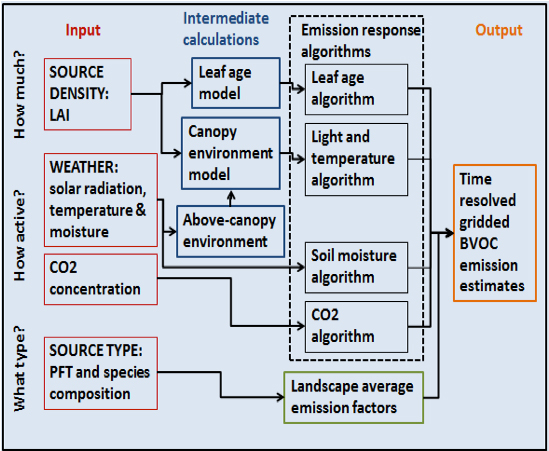
\includegraphics[width=\textwidth]{Figures/MEGANmodel_img.jpg}
        \caption{MEGAN schematic, copied from \citet{Megan_Website}}
        \label{Models:GC:Isop:MEGAN:fig_megan_schematic}
      \end{figure}
      
      MEGAN ``is a modelling framework for estimating fluxes of biogenic compounds between terrestrial ecosystems and the atmosphere to account for the major known processes controlling biogenic emissions.'' \citep{Guenther2012}.
      It allows parameterisation of various BVOC emissions, with descriptions given in \cite{Guenther2012}.
      Instructions to run version 2.1 are available at \url{http://lar.wsu.edu/megan/docs/MEGAN2.1_User_GuideWSU.pdf}, and a version using the Community Land Model (CLM) is available at \url{http://www.cesm.ucar.edu}.
      It uses meteorological fields from the Weather Research and Forecasting (WRF) modelling system.
      Version 2.1 (updated from 2.0 \citep{Guenther2006}) includes 147 species, in 19 BVOC classes, which can be lumped together to provide appropriate output for mechanisms in various chemical models.
      
      MEGAN was developed as a replacement for two earlier canopy-environment emission models (BIES and GEIA), and initially included a simple canopy radiative transfer model, which parameterised sun-lit and shaded conditions through a canopy.
      Early models didn't account for abiotic stresses, such as drought, prior rainfall and development processes, although these influenced species specific emissions by more than an order of magnitude \citep{Niinemets1999}.
      Isoprene emissions were based on temperature, leaf area, and light, but have since been updated to include leaf age activity \citep{Guenther2000}, and a leaf energy balance model \citep{Guenther2006} in MEGANv2.0.
      This update included a parameter for soil moisture, to account for drought conditions, however this parameter is currently (as of version 2.1) not applied to isoprene \citep{Sindelarova2014}.
      Soil moisture effects on isoprene emission are very important, and can drastically affect estimates.
      
      MEGAN has recently been analysed using 30 years of meteorological reanalysis information by \cite{Sindelarova2014}.
      They estimate emissions of Biogenic VOCs (BVOCs) to be 760~Tg(C)yr$^{-1}$, 70\% (532~Tg(C)yr$^{-1}$) of which is isoprene.
      This is similar to isoprene emission estimates from MEGAN itself, of 400-600~Tg(C)yr$^{-1}$ \citep{Guenther2006}.
      MEGAN emissions estimates are termed bottom-up, as opposed to top-down which are derived from satellite measurements of the products of various VOCs.
      Using GOME satellite HCHO and a Beyesian inversion technique to derive isoprene emissions, \cite{Shim2005} estimated global isoprene emissions to be $\sim566$~TgC yr$^{-1}$. 
      This estimate is greater than initially thought and leads to decreased ($\sim10\%$) simulated OH concentrations to 9.5e5 molec cm$^{-3}$.
      
      One of the important parameters in Australia is the soil moisture activity factor($\gamma_{SM}$), which can have large regional affects on the isoprene emissions \citep{Sindelarova2014,Bauwens2016}.
      Generally if soil moisture is too low, isoprene emissions stop \citep{Pegoraro2004,Niinemets2010}, however in many Australian regions the plants may be more adapted to lower moisture levels. (TODO: Find cites for this - talk from K Emerson at Stanley indicated this)
      GEOS-Chem runs MEGANv2.1, which has three possible states for isoprene emissions based on the soil moisture ($\theta$):
      \begin{align*}
        \gamma_\mathrm{SM} & = 1 && \theta > \theta_1 \\
        \gamma_\mathrm{SM} & = (\theta-\theta_w)/\Delta\theta_1  && \theta_w < \theta < \theta_1 \\
        \gamma_\mathrm{SM} & = 0 && \theta < \theta_w \\
      \end{align*}
      where $\theta_w$ is the wilting point, and $\theta_1$ determines when plants are near the wilting point.
      The wilting point is set by a land based database from \citet{Chen2001}, while $\theta_1$ is set globally based on \citet{Pegoraro2004}.
      
      In GEOS-Chem the isoprene emissions can be globally multiplied by a constant factor.
      By running the model two extra times, with the biogenic isoprene emissions turned off in one run and halved in another, while other parameters remain unchanged. 
      These modified runs allow an estimate of model sensitivity to isoprene emissions and smearing impact as described in Section \ref{BioIsop:Methods:Smearing}.
  
  \subsection{Chemical Mechanisms}
  \label{Model:GC:Mechanisms}
    Chemical reactions are turned into systems of differential equations (DEs) to be solved by the CPU for each gridbox in GEOS-Chem.
    Some of the important ones involving isoprene are copied here, including reaction rates in the form $ k = A \exp{-ER/T} $.
    
    \begin{align} \begin{split}
      \label{Model:GC:Mechanisms:eqn_mechanisms}
      \ce{
        RIO2 + NO ->[2.7*10^{-12} \exp{350/T}] & .883NO2 + .783HO2 + .66CH2O \\
         & + .4MVK + .26MACR + .07ISOPND \\
         & + .123HC5 + .1DIBOO \\
        RIO2 ->[4.07*10^{8} \exp{-7694/T}] & 2HO2 + CH2O + .5MGLY + .5GLYC \\
         & + .5GLYX + .5HAC + OH
      }
%     % k1=2.7*10^{-12} \exp{350/T}
%     % k2=4.07*10^{8} \exp{-7694/T}
%      
    \end{split} \end{align}
  
  \subsection{Running GEOS-Chem (before isop?)}
  \label{Model:GC:running}
    \subsubsection{Installation and requirements}
      GEOS-Chem instructions for download, compilation, and running can be found in the user guide provided by Harvard: \url{http://acmg.seas.harvard.edu/geos/doc/man/}.
      In order to build and run GEOS-Chem a high-speed computing system is optimal, as globally gridded chemical calculations can take a long time to perform.
      I installed GEOS-Chem onto a suitably configured workspace on the National Computational Infrastructure (NCI, \url{http://nci.org.au/}). 
      This workspace included access to compilers and libraries which are needed to build the Fortran based GEOS-Chem source code, and IDL, Python, and various editors and scripting languages to read, run, edit, and analyse both GEOS-Chem and its output.
        
      After downloading GEOS-Chem, the code can be compiled with different options for resolution and chemical mechanisms.
    \subsubsection{Options}
    
    \subsubsection{Tropospheric chemistry run}
    
    \subsubsection{UCX run}
    % TODO: layout reasons why isoprene differs between runs
    %    In GeosCore/fast_jx_mod.F:
    %      strat aerosols are scaled somehow at line 2922, looks like it affects SSA.
    %      line 4138: comment says ozone calculated online.
    %	  TOMS/SBUV O3 are read by toms_mod.f, passed to FAST-J routine ``set_prof.f''. in UCX the stratospheric O3 is calculated online
    %    In GeosCore/calcrate.F:
    %      line 1489 comment says rates are limited to prevent solver failure
    %	if lifetime of A is below PSCMINLIFE, limit reaction rate to yield the specified lifetimedepletion
    %      Line 1724
    %        ! SPECIAL TREATMENT FOR O3+hv -> OH+OH (trop-only simulation)
    %        !                    or O3+hv -> O+O2  (UCX simulation)
    %      line 1752:
    %      #if defined( UCX )
    %        IF ( NKO3PPHOT(NCS) > 0 ) THEN
    %          PHOTVAL_2 = NKO3PPHOT(NCS) - NRATES(NCS)
    %          NKN_2     = NKNPHOTRT(PHOTVAL_2,NCS)
    %        ENDIF
    %      #endif
    %      line 1771:
    %        comment: change rate of O(1D) + N2 to 3.1e-11 at 298K (from 2.6e-11)...
    %        if not defined UCX:
    %	  RO1Dp1H2O, RO1Dp1H2, RO1D, (and maybe 2 RRates) are changed.
    
    \subsection{Run comparisons}
    
      There are many options available when running GEOS-Chem depending on the desired chemistry, resolution, meteorology, and boundary conditions.
      Here we compare the model output with and without enabling the Universal tropospheric-stratospheric Chemistry eXtension (UCX).
      %From version 11 of GEOS-Chem, the UCX mechanism is enabled by default.
      Both runs use 2$^{\circ}$ latitude by 2.5$^{\circ}$ longitude, however the UCX mechanism is run with 72 vertical levels from the surface to the top of the atmosphere (TOA$\sim$0.1~hPa), while the standard (tropchem) run uses 47 levels.
      The extra vertical levels are added in the stratosphere, providing finer vertical resolution from around 70~hPa to the top of the atmosphere.
      For both runs the inpup parameters such as MEGAN emissions and GEOS-5 meteorological fields are identical.
      
      GEOS-Chem output of HCHO does not differ much between runs with or without the Unified Chemistry eXchange (UCX).
      Figure \ref{Model:GC:running:fig_UCXvsTrop_HCHO} shows an example of surface HCHO amounts with and without UCX turned on.
      The differences do not exceed 3\% over Australia for the averaged month of January, 2005.
      
      \begin{figure}%[!htbp] % TODO: remove 'rerun' plot, use normal and delete rerun thingy so it's not confusing later.
        % These figures created in GC_test.py -> TODO:
        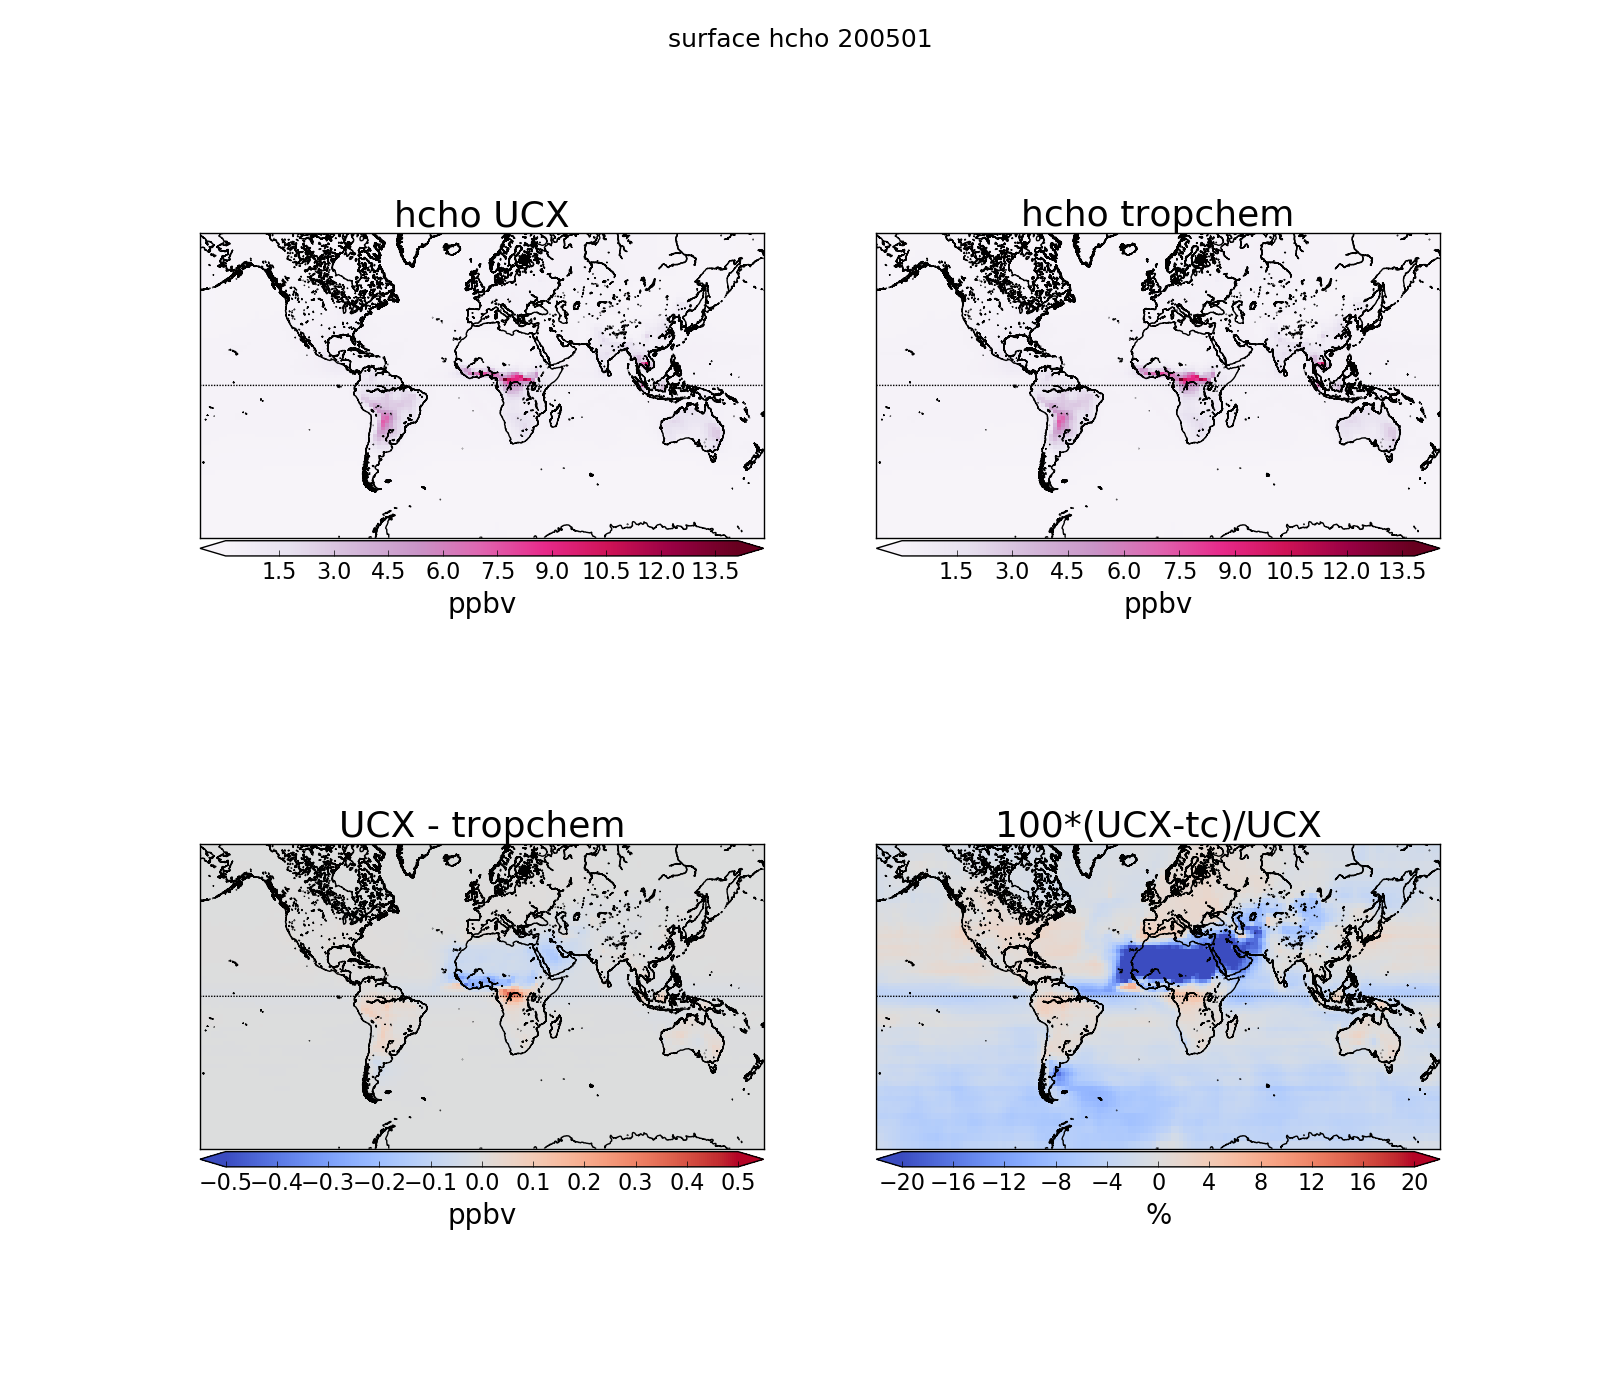
\includegraphics[width=\textwidth]{Figures/OMI_link/GC/UCX_vs_trp_glob_200501_hcho_rerun.png}
        \caption{ %
          Surface HCHO simulated by GEOS-Chem with UCX (top left), and without UCX (top right), along with their absolute and relative differences(bottom left, right respectively).
          Amounts simulated by GEOS-Chem for the 1st of January, 2005.
        }
        \label{Model:GC:running:fig_UCXvsTrop_HCHO}
      \end{figure}
      
      Figure \ref{Model:GC:running:fig_UCXvsTrop_Isop} shows the differences in surface isoprene amounts over Australia.
      Here we start to see a higher relative difference in concentrations, although this is generally over the areas with less absolute concentrations. 
      Very little isoprene is seen away from the continent (4-5 orders of magnitude less), due to the short lifetime of isoprene, and lack of emissions over the oceans.
      Generally isoprene is 0-30\% higher over Australia when the UCX mechanism is turned on.
      This enhancement can be seen throughout the entire tropospheric column as shown by Figure TODO fix ref \ref{ch_HCHO:fig:isoptropUCXcomparison}. %TODO: fix ref
      \begin{figure}%[!htbp]
        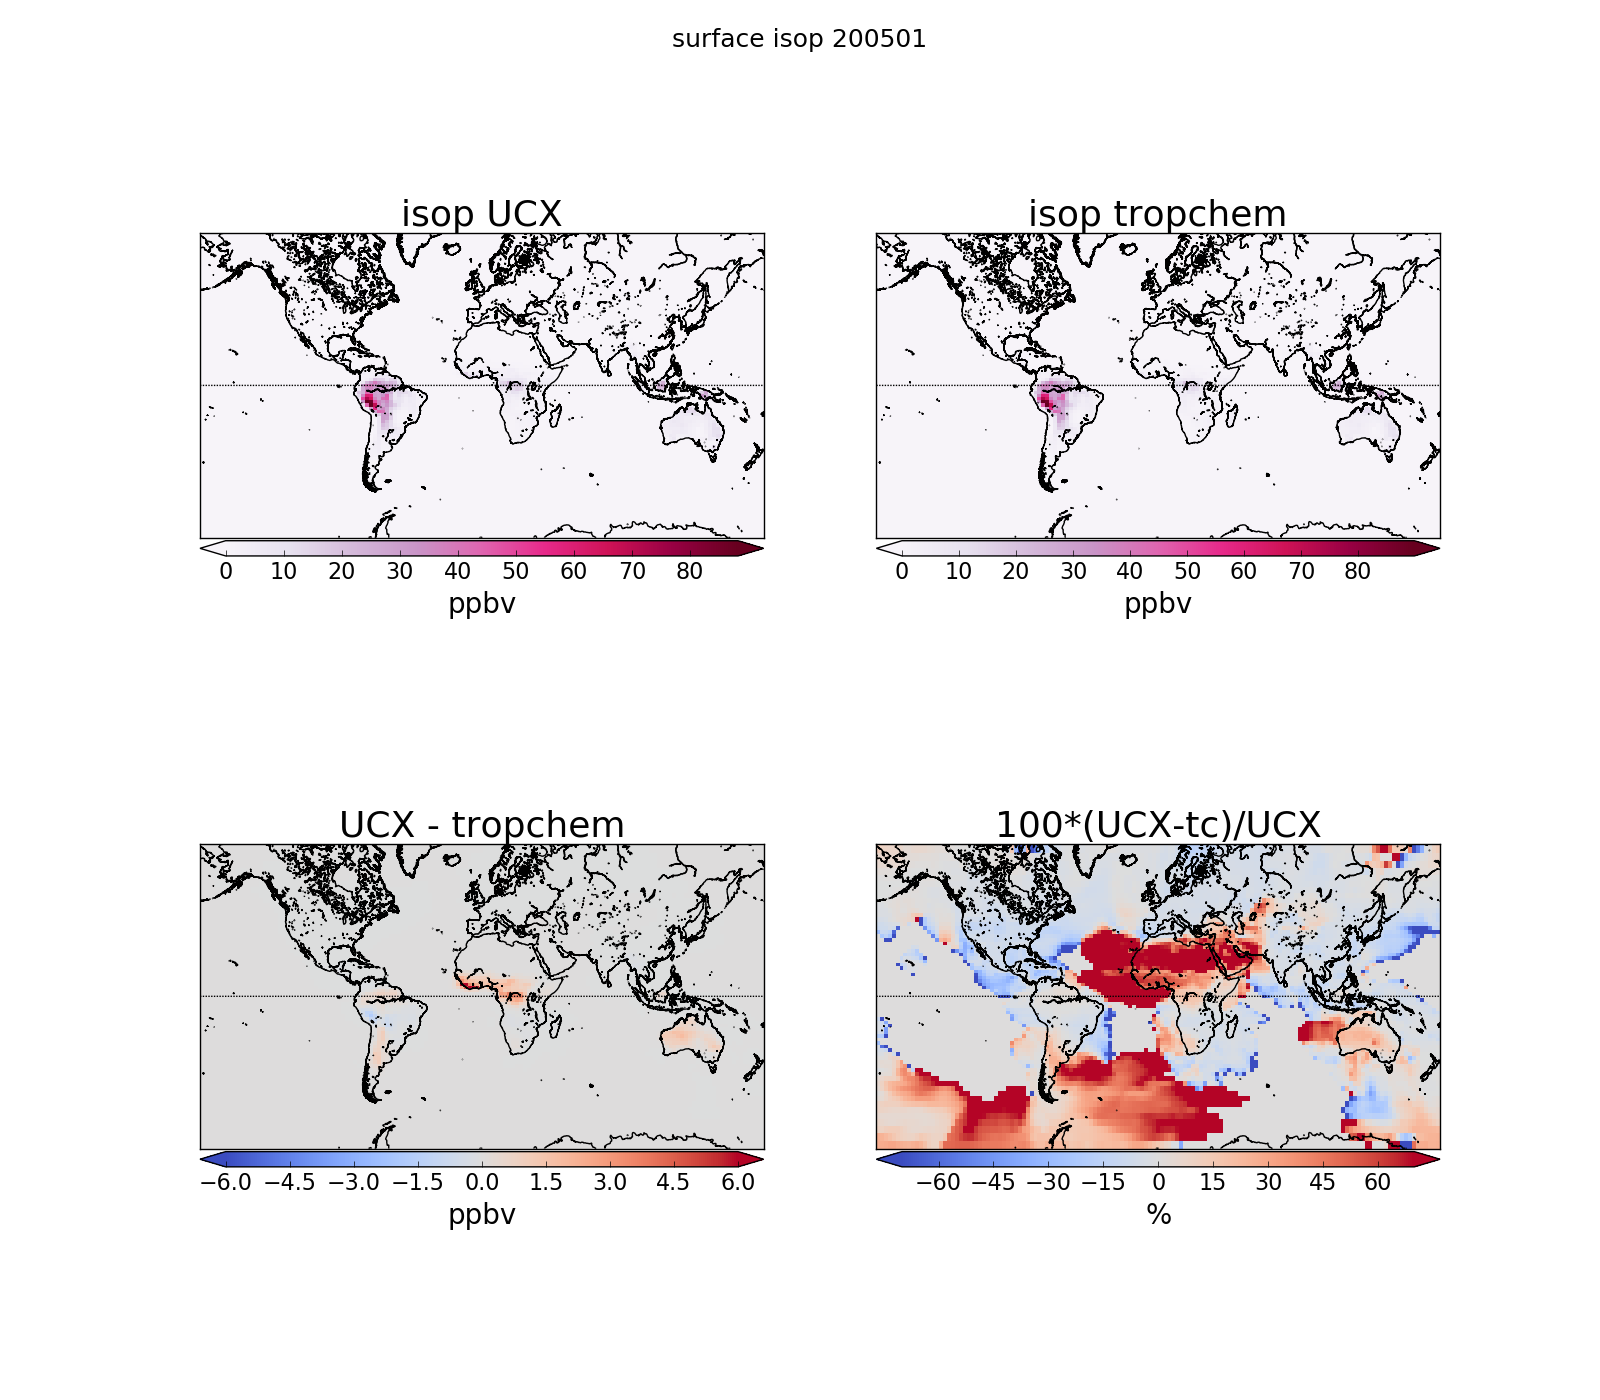
\includegraphics[width=\textwidth]{Figures/OMI_link/GC/UCX_vs_trp_glob_200501_isop_rerun.png}
        \caption{ %
          As figure \ref{Model:GC:running:fig_UCXvsTrop_HCHO}, except looking at isoprene. 
        }      
        \label{Model:GC:running:fig_UCXvsTrop_Isop}
      \end{figure}
      
      
      Figure TODO: shows the columns for isoprene and HCHO simulated by our two mechanisms over Australia in January of 2005.
      The differences are minimal compared to other uncertainties in both AMF calculation and emissions estimation.
      
      
      TODO: The difference in isoprene between UCX and tropchem is likely caused by differences in the modelled radiation reaching the troposphere due to differences in simulated ozone in the stratosphere.
      With higher stratospheric ozone levels, less radiation would reach the troposphere, changing the photochemistry.
      Figure \ref{Model:GC:running:fig_UCXvsTrop_O3} shows the total column ozone between UCX and non-UCX runs, we can see that UCX has TODO: less or more ozone over Australia/USA in January.
          
      \begin{figure}%[!htbp]
        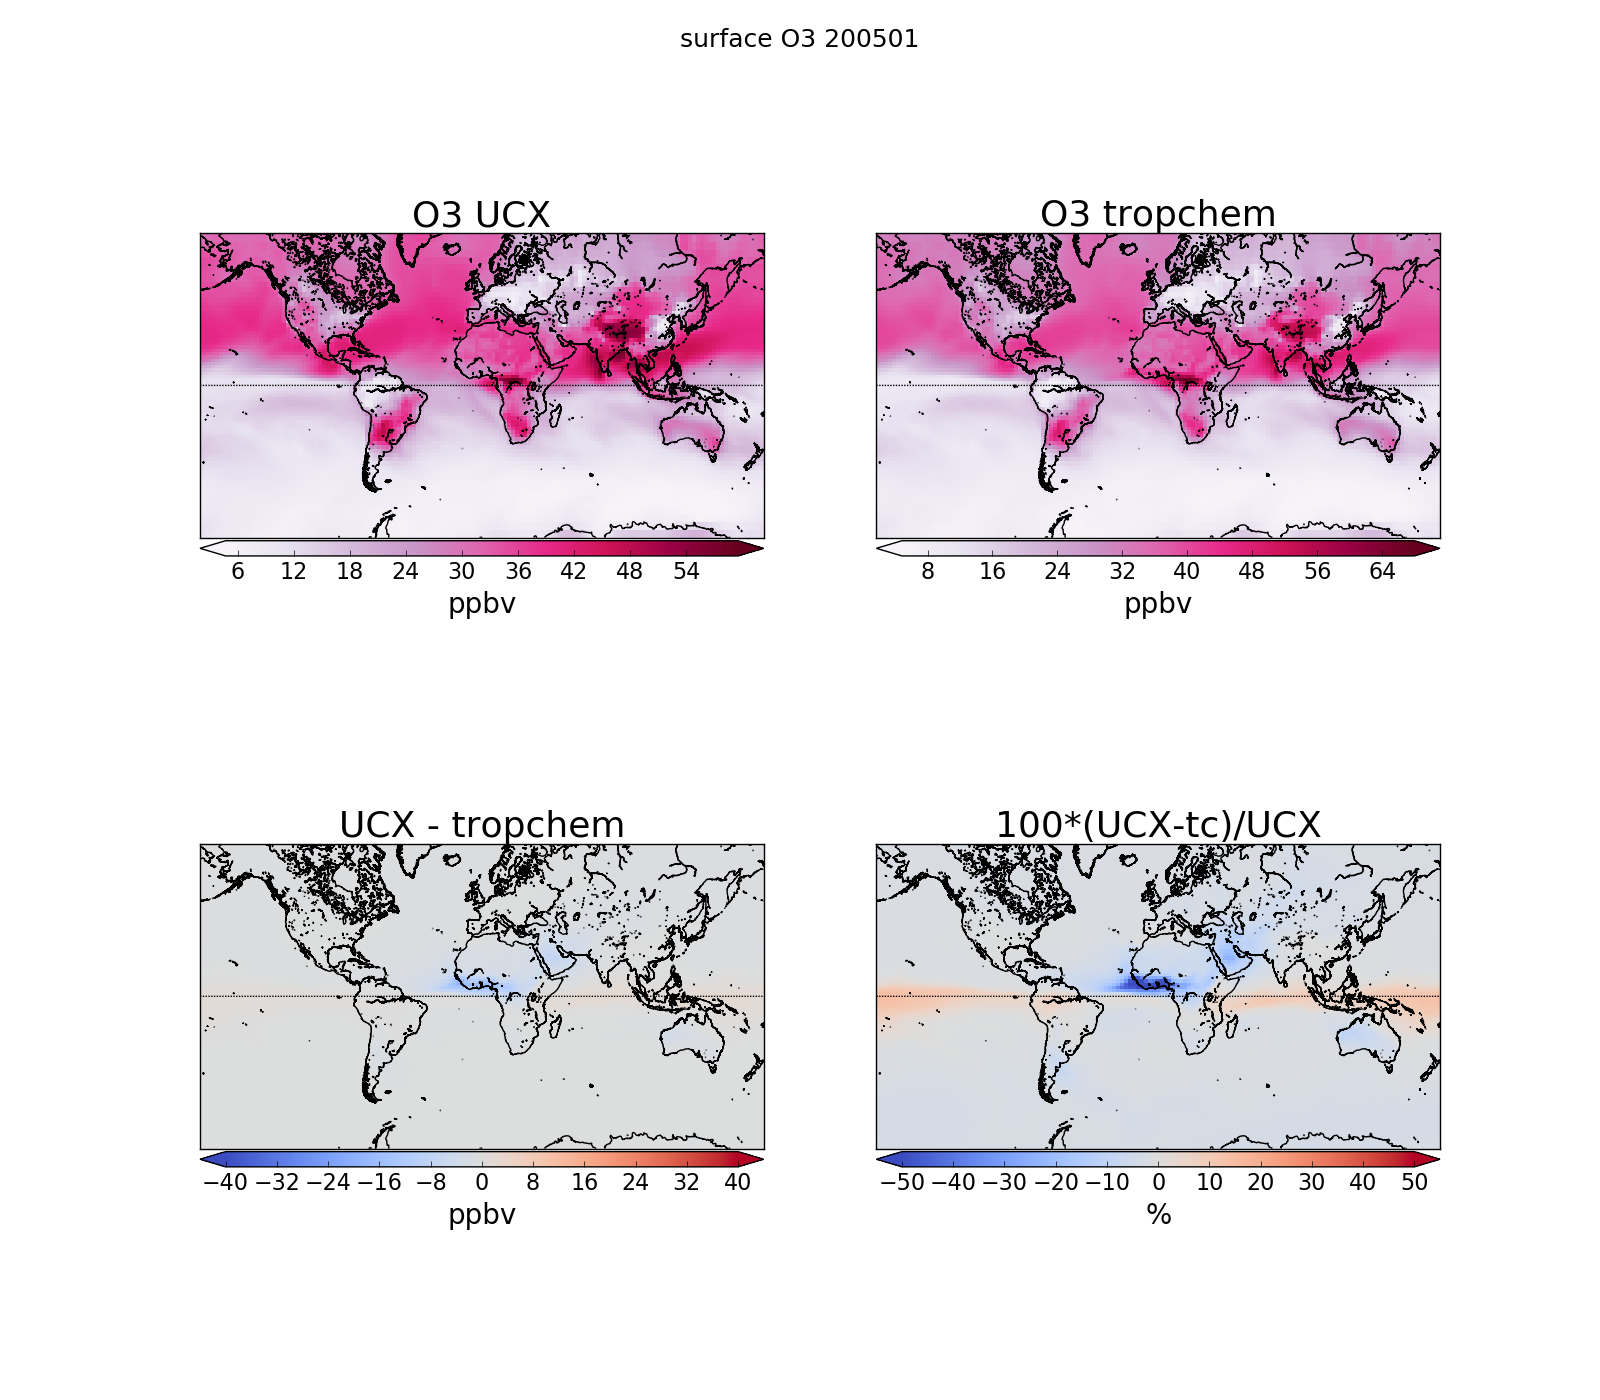
\includegraphics[width=\textwidth]{Figures/OMI_link/GC/UCX_vs_trp_glob_200501_O3_rerun.png}
        \caption{%
          As figure \ref{Model:GC:running:fig_UCXvsTrop_HCHO}, except looking at ozone. 
        }
        \label{Model:GC:running:fig_UCXvsTrop_O3}
      \end{figure}

\section{CAABA/MECCA}
\label{Model:CM}
  
  CAABA (Chemistry As A Boxmodel Application) estimates the chemical concentrations accounting for J-values (JVAL), simplified and parameterised photolysis (SAPPHO) and simplified emission and depositions (SEMIDEP).
  CAABA runs in a single scenario (or box) with given emissions, depositions, and initial concentrations, allowing the examination of chemistry in a very specific environment to be modelled with high temporal resolution.
  
  This has been used with an atmospheric chemistry model MECCA (Module Efficiently Calculating the Chemistry of the Atmosphere) which implements tropospheric and stratospheric chemistry for both the gas and the aqueous phases \citep{Sander2005}.
  MECCA chemical mechanisms include basic O$_3$, CH$_4$, NO$_X$, and HO$_X$ chemistry, as well as non methane hydrocarbon (NMHC) chemistry, considering gas phase, aqueus phase, and heterogenous reactions. \citep{Sander2005}
  For the numerical integration, MECCA uses the KPP software (\cite{SanduSander2006}), which takes chemical reactions and their rate coefficients and codes integral solutions to the system.
  The combination of the CAABA box model with MECCA module is called CAABA/MECCA and is currently at version 3.
  CAABA/MECCA been implemented for various calculations including ozone chemistry throughout the atmosphere in \cite{Zanis2014}.
  
  MECCA could also be used as the chemistry mechanism for a more complex, 3-dimensional model (\cite[e.g.][]{Jockel2006}).
  The connection is established via the MESSy interface (\url{http://www.messy-interface.org}) developed by \cite{Jockel2005} as part of an effort to simplify the framework for modelling the atmospheres at various scales.
  The user manual is available online at \url{http://www.rolf-sander.net/messy/mecca/caaba_mecca_manual.pdf}.


\section{Measurement Techniques}
  \label{Model:Meas}
  While I have not made any measurements myself, it is important to understand the techniques used in datasets I have utilised in order to understand possible anomalous datapoints or trends.
  
  % Measurement difficulties
  In-situ measurements contain errors, and depending on the device used and chemical being measured this error can be significant.
  \cite{Dunne2017} analyse the uncertainty of VOC measurements (including isoprene) using three different techniques during a campaign in Sydney in 2012.
  The major sources of uncertainty in measurement techniques included interference from non-target compounds and under-reporting.
  Overall isoprene uncertainty in their measurements was a factor of 1.5 to 2.
  This can feed into uncertainties in modelling and satellite retrievals, as verification and correlations are affected.
  
  \subsection{DOAS}
  
    %TODO: is some of this is repeated in isoprene chapter satellite section.
    The DOAS technique uses solar radiation absorption spectra to measure trace gases through paths of light.
    Beer's law states that $ T = I/I_0 = e^{-\tau} $ with T being transmittance, $\tau$ being optical depth, and I, I$_0$ being radiant flux received at instrument and emitted at source respectively.
    From $ \tau_i = \int \rho_i \beta_i ds $ we get:
    $$ I = I_0 \exp {\left( \Sigma_i \int \rho_i \beta_i ds \right) } $$
    Where i represents a chemical species index, $\rho$ is a species density(molecules per cm$^3$), $\beta$ is the scattering and absorption cross section area (cm$^2$), and the integral over ds represents integration over the path from light source to instrument.
    
    Generally satellites use a DOAS based technique, with chemical transport and radiative transfer models used to transform the non-vertical light path interference into vertical column amounts.
    
    Multiple axis DOAS (MAX-DOAS) is a remote sensing technique which uses several DOAS measurements over different viewing paths.
    In these retrievals, the measurements of light absorption are performed over several elevations in order to add some vertical resolution to the measurement of trace gas concentrations.
    An example of this is shown in figure \ref{LR:HCHO:fig_MAXDOASExample}, which was taken from \cite{Lee2015}.
    Recently MAX-DOAS has been used to examine HCHO profiles in the clean free troposphere (\cite{Franco2015, Schreier2016}) as well as in polluted city air (\cite{Lee2015}).
    Depending on orography and atmospheric composition (ie. the influence of interfering chemicals), MAX-DOAS can be used to split the tropospheric column into two partial columns; giving a small amount of vertical resolution to HCHO measurements \citep[eg.]{Franco2015, Lee2015}.
    In \cite{Franco2015}, an FTIR spectrometer at Jungfraujoch is compared against both MAX-DOAS and satellite data, with two CTMs; GEOS-Chem and IMAGES v2 used to compare total columns and vertical resolution of each instrument.
    
    \begin{figure}
      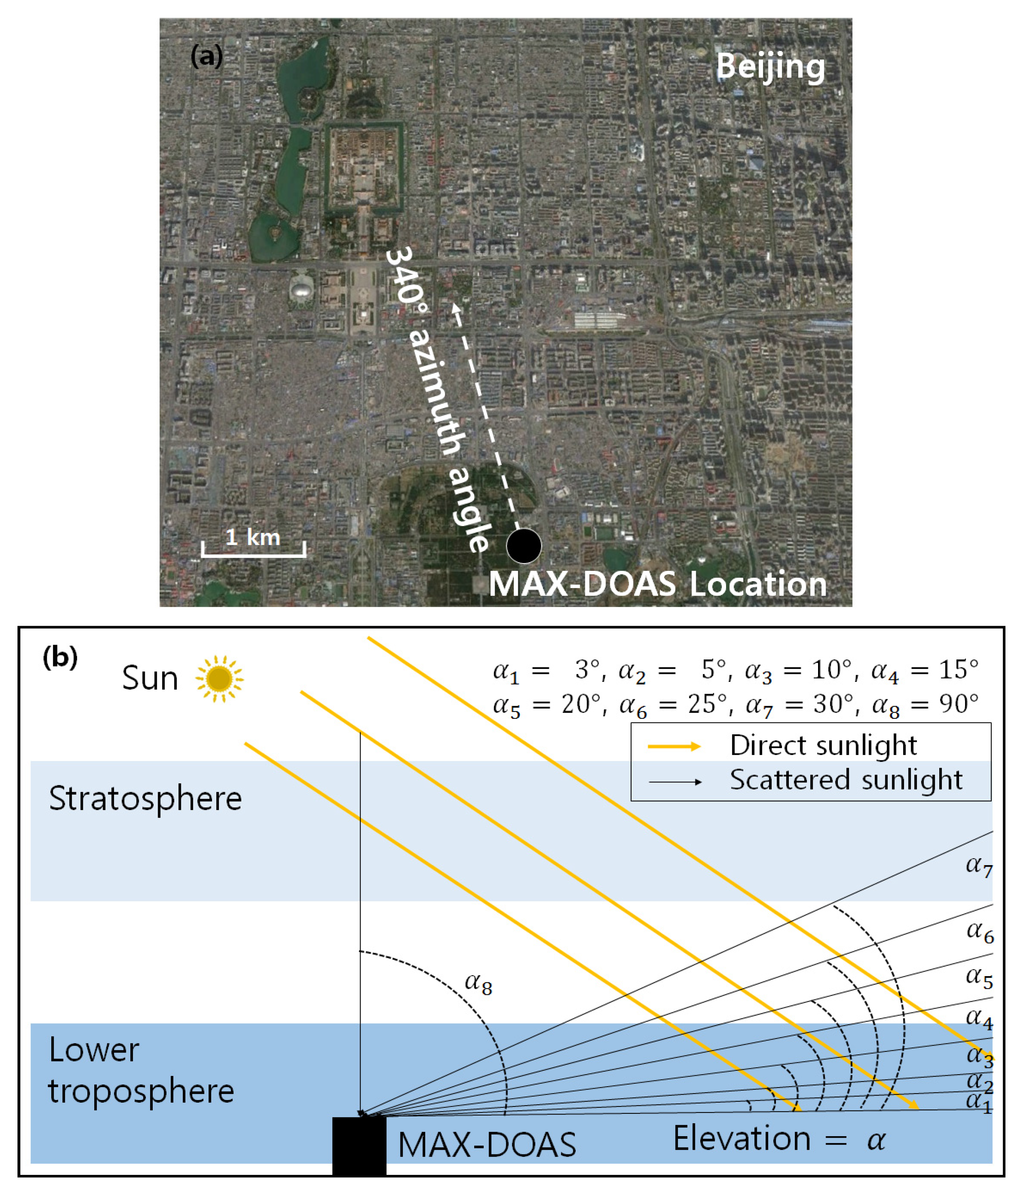
\includegraphics[width=\textwidth]{Figures/MAXDoasExample.png}
      \caption{ Image from \cite{Lee2015}.}
      \label{LR:HCHO:fig_MAXDOASExample}
    \end{figure}
    
  \subsection{Satellites}
  \label{Model:Meas:sat}
    Measurements done using DOAS often apply a forward radiative transfer model (RTM) such as LIDORT in order to determine a trace gas's radiative properties at various altitudes.
    The forward RTM used for satellite data products also involves functions representing extinction from Mie and Rayleigh scattering, and the efficiency of these on intensities from the trace gas under inspection, as well as accounting for various atmospheric parameters which may or may not be estimated (e.g. albedo).
    
    Satellites record near nadir (vertical) reflected spectra between around 250-700~nm split into spectral components at around $0.3$~nm in order to calculate trace gases including O$_3$, NO$_2$, and HCHO (eg: \cite{Leue2001}).
    Several public data servers are available which include products from satellites, including NASAs Earthdata portal (\url{https://earthdata.nasa.gov/}) and the Belgian Institute for Space Aeronomy (IASB-BIRA) Aeronomie site (\url{http://h2co.aeronomie.be/}).
    
    Satellite measurements are generally performed using spectral fitting followed by conversion to vertical column densities.
    The use of multiple satellites can even be used to detect intradiel concentrations in trace gas columns, as shown in \cite{Stavrakou2015} using OMI and GOME-2 measurements, which have respective overpass times of 1330 and 0930 LT.
    Instruments including MODIS on board the AQUA and TERRA satellites are also able to determine aerosol optical depth (AOD), a measure of atmospheric scatter and absorbance. 
    An AOD of under 0.05 indicates a clear sky, while values of 1 or greater indicate increasingly hazy conditions.
    This is important in order to determine where measurements from other instruments may be compromised by high interference.
    Satellite measured AOD requires validation by more accurate ground based instruments like those of AERONET which uses more than 200 sun photometers scattered globally.
    
    Soon even more HCHO data will be available in the form of geostationary satellite measurements (\cite{Kwon2017}).
    \cite{Kwon2017} examine simulated geostationary measurements against GEOS-Chem column simulations to determine the most important instrument sensitivities.
    Geostationary satellites can provide temporally rich measurements over an area, as they are not sweeping around the earth but fixed relative to one latitude and longitude.
    
    \subsubsection{OMI}
    
      The OMI instrument on board AURA has been active since July 2005, it records spectra from 264-504~nm using an array of 60 detectors with mid-resolution (0.4-0.6~nm).
      This band of wavelengths allows measurments of trace gases including O$_3$, NO$_2$, SO$_2$, HCHO, and various other quantities like surface UV radiation.
      Recently \cite{Schenkeveld2017} analysed the performance over time of the instrument and found irradiance degradation of 3-8\%, changed radiances of 1-2\%, and a stable wavelength calibration within 0.005-0.020~nm.
      They also provide a very nice summary of the OMI instrument copied here in Fig. \ref{LR:HCHO:Sat:fig_Shenkeveld_OMI_summary}, as it shows the instruments spectral, temporal, and spatial resolutions.
      These changes are measured excluding the row anomaly (RA) effect, which is relatively stable since 2011, although it is still growing and remains the most serious concern.
      An analysis of the row anomaly by \cite{Huang2017} state that OMI ozone columns remain suitable for scientific use, with recommendation for further evaluation.
      And analysis of OMI output by \cite{Schenkeveld2017} concludes that data is still of high quality and will deliver useful information for 5-10 more years, with radiances only changing by $1-2\%$ outside of RA impacted areas.
      The RA began in June 2007, with some cross-track rows seemingly blocked. The most likely cause is some instrument insulation partially obscuring the radiance port (\cite{Schenkeveld2017}).
      
      \begin{figure}
        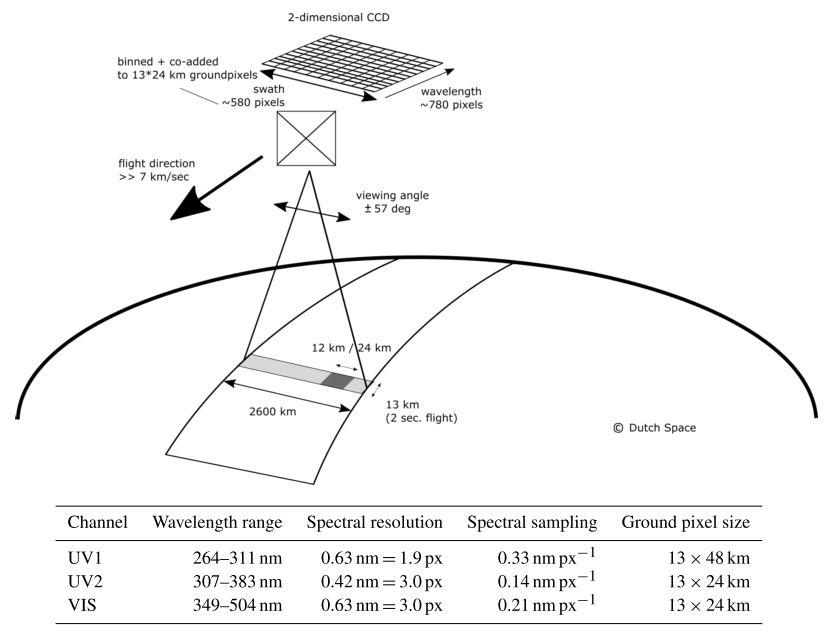
\includegraphics[width=\textwidth]{Figures/Shenkeveld_OMI_summary.png}
        \caption{ %
          Figure 1 and Table 1 from \cite{Schenkeveld2017}, with the following caption ``An impression of OMI flying over the Earth.
          The spectrum of a ground pixel is projected on the wavelength dimension of the charge-coupled device (CCD; the columns). 
          The cross-track ground pixels are projected on the swath dimension of the CCD (the rows).
          The forward speed of 7~kms$^{-1}$ and an exposure time of 2~s lead to a ground pixel size of 13~km in the flight direction.
          The viewing angle of 114\degr leads to a swath width on the ground of 2600~km.''
          The table shows the optical properties for OMIs three channels.}
      \label{LR:HCHO:Sat:fig_Shenkeveld_OMI_summary}
      \end{figure}
        
    \subsubsection{AMF}
      To convert the trace gas profile from a reflected solar radiance column (slanted along the light path) into a purely vertical column requires calculations of an air mass factor (AMF).
      In satellite data, the AMF is typically a scalar value for each horizontal grid point which will equal the ratio of the total vertical column density to the total slant column density.
      This value requires calculations to account for instrument sensitivities to various wavelengths over resolved altitudes, and is unique for each trace gas under consideration.
      
      An AMF characterises measurement sensitivity to a trace gas at various altitudes \cite[e.g.]{Palmer2001}.
      \cite{Lorente2017} show that AMF calculations can be the largest source of unertainty in satellite measurements.
      Another way of describing AMFs are as measures of how radiance at the top of the atmosphere (TOA) changes with trace gas optical depths at specific altitudes (\cite{Lorente2017}).
      Calculation of the AMF is important as it is multiplied against the estimated slant columns in order to give vertical column amounts.
      
      Related to the AMF is the averaging kernal (AK), which is used to handle instrument measurements which are sensitive to concentrations at different altitudes in the atmosphere.
      DOAS methods can be heavily influenced by the initial estimates of a trace gas profile (the apriori) which is often produced by modelling, so when comparing models of these trace gases to satellite measurements extra care needs to be taken to avoid introducing bias from differing apriori assumptions.
      One way to remove these apriori influences is through the satellites AK (or by using AMFs), which takes into account the vertical profile of the modelled trace gas and instrument sensitivity to the trace gas (\cite{Eskes2003, Palmer2001}).
      % TODO read and note this paper:
      \cite{Lamsal2014} recommends that when comparing satellite data to models, the AMF should first be recalculated using the model as an apriori.
      This is in order to remove any apriori bias between model and satellite columns.
      
    \subsubsection{Uncertainties}
      %Satellite Errors
      While satellite data is effective at covering huge areas (the entire earth) it only exists at a particular time of day, is subject to cloud cover, and generally does not have fine horizontal or vertical resolution.
      Concentrations retrieved by satellites have large uncertainties, which arise in the process of transforming spectra to total column measurements, as well as instrument degradation (satellite instruments are hard to tinker with once they are launched).
      Uncertainty in transforming satellite spectra comes from a range of things, including measurement difficulties introduced by clouds, and instrument sensitivity to particular aerosols \citep{Millet2006}.
      Many products require analysis of cloud and aerosol properties in order to estimate concentration or total column amounts \citep{Palmer2001,Palmer2003, Marais2012, Vasilkov2017}.
      The main source of error in satellite retrievals of HCHO are due to instrument detection sensitivities, and the vertical multiplication factor (discussed in more detail in Section \ref{BioIsop:Uncertianty:Satellite}) \citep{Millet2006}.
      
      There are two types of measurement error, arguably the worst of these is systematic error (or bias) which normally indicates a problem in calculation or instrumentation.
      If the systematic error is known, it can be corrected for by either offsetting data in the opposite direction, or else fixing the cause.
      A proper fix can only be performed if the sources of error are known and there is a way of correcting or bypassing it.
      Random error is the other type (often reported as some function of a datasets variance, or uncertainty), and this can be reduced through averaging either spatially or temporally. 
      By taking the average of several measurements, any random error can be reduced by a factor of one over the square root of the number of measurements.
      This is done frequently for satellite measurements of trace gases (which are often near to the detection limit over much of the globe).
      For example: \cite{Vigouroux2009} reduce the measurement uncertainty (in SCIAMACHY HCHO columns) by at least a factor of 4 through averaging daily over roughly 500km around Saint-Denis, and only using days with at least 20 good measurements.
      
      %% grid size and averaging
      Satellite measurements of HCHO are relatively uncertain, however this can be improved by averaging over larger grid boxes or longer time scales.
      An example of this can be seen in \cite{Dufour2009}, where monthly averaging is used to decrease the measurements uncertainty.
      They examine HCHO in Europe, which is low; near the detection limit of satellite measurements.
      Taking monthly averages allows enough certainty that useful inversions can be determined to estimate the source emissions of HCHO.
      The finer nadir resolution of OMI (13 by 24~km${^2}$) compared to other satellites reduces cloud influence (\cite{Millet2006, Millet2008}). 
      Although the uncertainty in each pixel is $\sim 2 \times 10^{16}$, which is $5 \times$ higher than GOME, there are $\sim 100-200 \times $ as many measurements due to the smaller footprint and better temporal resolution of OMI, which allows a greater reduction of uncertainty with averaging (\cite{Chance2002,Millet2008}).
      
      %% SURFACE CONDITIONS AND CLOUDS
      In cloudy, hazy or polluted areas measurements are more difficult to analyse (\cite[e.g.][]{Palmer2003,Marais2014}).
      Recent work by \cite{Vasilkov2017} showed that updating how the surface reflectivity is incorporated into satellite measurements can change the retrievals by 50~\% in polluted areas.
      
      %% BACKGROUND MEASUREMENTS
      In satellite HCHO products, concentrations over the remote pacific ocean are sometimes used to analyse faulty instrument readings.
      This is due to the expected invariance of HCHO over this region.
      For instance GOME (an instrument which measures trace gases on board the ERS-2) corrects for an instrument artifact using modelled HCHO over the remote pacific (\cite{Shim2005}).
      OMI HCHO products use a similar technique to account for sensor plate drift and changing bromine sensitivity (\cite{Abad2015})
      
      
      %% EXAMPLES OF BIAS
      For many places the tropospheric column HCHO measured by satellite is biased low, \cite{Zhu2016} examine six available datasets and show a bias of 20 - 51\% over south east USA when compared against a campaign of aircraft observations (SEAC$^4$RS).
      \cite{DeSmedt2015} also found a low bias from 20 - 40\% when comparing OMI and GOME2 observations against ground based vertical profiles, and \cite{Barkley2013} determine OMI to be 37\% low compared with aircraft measurements over Guyana.
      These bias can be corrected by improving the assumed apriori HCHO profiles which are used to calculate the AMFs of the satellite columns.
      \cite{Millet2006} examine OMI HCHO columns over North America and determine overall uncertainty to be 40\%, with most of this coming from cloud interference.
      \cite{Millet2008} shows that there also exists some latitude based bias, as well as a systematic offset between the OMI and GOME instruments.
      This does not appear to be due to the different overpass times of the two instruments.
      
      %% UNCERTAINTY CALCULATIONS
      Uncertainty in the OMI satellite instrument is calculated by the Smithsonian Astrophysical Observatory (SAO) group using the uncertainty in backscattered radiation retrievals (\cite{Abad2015, Abad2016}).
      Another method of calculating the uncertainty is used by the Belgian Institute for Space Aeronomy (BIRA) group, who determine uncertainty from the standard deviation of HCHO over the remote pacific ocean \citep{DeSmedt2012, DeSmedt2015}.
      
      A full analysis of the AMF uncertainty in OMI measurements, as well as the structural uncertainty (between different systems of calculations applied to the same data) is performed by \cite{Lorente2017}.
      They determine the structural uncertainty using ensemble techniques on seven AMF calculation approaches used by different retrieval groups.
      They show that in scenarios where the gas is enhanced in the lower troposphere, AMF calculation is the largest uncertainty in satellite measurements.
      In polluted environments the structural uncertainty is estimated at 42~\%, or 31~\% over unpolluted environments.
      The importance of apriori and ancilliary data (such as surface albedo and cloud top height) is also shown, as it sharply affects the structural uncertainty.
      
      GOME suffers from similar uncertainties to OMI, as the same general method of DOAS remote measurements are performed.
      The uncertainty from slant column fitting has been calculated for GOME to be $4\times10^{15}$ molecules cm$^{-2}$ \citep{Chance2000, Millet2006}. 
      The conversion factor for slant to vertical columns (AMF) calculation also suffers from errors; primarily from surface albedo, HCHO vertical profile apriori, aerosol, and cloud influence \citep{Millet2006}. 
      AMF uncertainties for GOME are calculated to be $1$ to $1.3\times10^{15}$ molecules cm$^{-2}$ by \cite{Shim2005}.
  

\section{Campaigns and datasets}
  \label{Model:Datasets}
  Here I will describe the various datasets I've used to analyse GEOS-Chem output.
  These datasets are also used to determine how suitable GEOS-Chem is in calculation of isoprene emissions estimations in chapter \ref{BioIsop} and ozone transport extrapolations in chapter \ref{Ozone}.
  
  TODO: these summaries.
  
  %Omi summary
  \subsection{OMI Satellite measurements}
  \label{Model:Datasets:OMI}
  
    \subsubsection{OMI HCHO}
    Recalculated OMI formaldehyde columns are used as a basis for estimating isoprene emissions in Chapter \ref{BioIsop}
    
    HCHO has been found to be biased low in several studies \cite[eg.][]{Zhu2016,DeSmedt2015,Barkley2013}
  
    \subsubsection{OMI NO2}
    \label{Model:Datasets:OMNO2d}

  Daintree summary (P. Nelson)
  
  % TODO: MUMBA summary
  \subsubsection{Marine and Urban MBA ? (MUMBA)}
    \label{Model:Datasets:MUMBA}
  
  \subsubsection{Sydney Particle Studies (SPS1, SPS2)}
    \label{Model:Datasets:SPS}
    Two VOC and other trace gas measurement campaigns took place at the Westmead Air Quality Station scientists from CSIRO, OEH, and ANSTO. 
    Stage 1 (SPS1) was from 5 February to 7 March in 2011, while stage 2 (SPS2) ranged from 16 April to 14 May 2012.
    
    Two instruments measured VOC concentrations: one was a Proton transfer reaction mass spectrometer (PTR-MS), the other a gas chromatographer (GC) with an equipped flame ionisation detector (FID).
    The PTR-MS uses chemical ionisation mass spectrometry and can quantify VOCs at high temporal resolution ($< 1$~s).
    It was calibrated several times per day against hcho, isoprene, $\alpha$-pinene, and several more VOCs. Further details can be found in \cite{Dunne2012,Dunne2017} (TODO: Check papers).
    The output lists hourly averaged ppbv concentrations of trace gases based on the mass to charge ratio (m/z), which for isoprene is 69.
    It's possible that other chemicals (such as Furan, with the same m/z) interfered with this value, especially at low ambient isoprene concentrations and towards the end of autumn (SPS2) when wood fires usage starts to become frequent (TODO cite something).
    The GC-FID analysed samples collected in multi-absorbent tubes, with lower temporal resolution but no interferences. GC-FID data is averaged from 0500-1000~LT, and 1100-1900~LT. Further details for this method can be found in TODO: cite Min et al 2016.
    
    Figure TODO: shows isoprene and formaldehyde over the course of these two campaigns, as well as the detection limits (dashed lines), as measured by PTR-MS. In order to compare with GEOS-Chem output a daily average and an overpass time (1200-1300 LT) average are both created from these data.
    In averaging, any measurements below the machine detection limit are set to half of the detection limit, as done in (TODO: doi:10.5194/acp-15-223-2015, 2015) which should minimise any introduced bias.

\section{Analysing output}
\label{Model:Analysis}
  
  \subsection{Circadian emissions cycle}
    HEMCO diagnostics provide the simulated MEGAN isoprene emissions at high temporal resolution.
    TODO: Figure X shows the daily emissions cycles for a few regions over each season. 
    The regions are labelled in the top panel, and seasonally averaged emissions from grid-boxes in each region are shown below.
    TODO: Figure XX shows the emissions from SPS1 and 2 compared against GEOS-Chem estimates in the same grid square.
    
  \subsection{HCHO: Simulated vs Measured}
  \label{Model:Analysis:HCHO}
    
    HCHO precursors are heavily tied to temperature (TODO:cite), and model output shows how higher temperature leads to an increase in HCHO levels.
    Figures \ref{Model:Analysis:HCHO:fig_hcho_vs_temp_SEA_200501} - \ref{Model:Analysis:HCHO:fig_hcho_vs_temp_SWA_200501} show the relationship between temperature and HCHO, for January 2005, within subsets of Australia.
    A reduced major axis regression is used to determine the linear slopes between surface temperature (X axis) and HCHO (Y axis).
    This gives us a linear regression for each region however it's clear from the straight line and from literature that the relationship is not linear but rather exponential (TODO: cite and example studies).
    Using the natural log of HCHO we can take the linear regression and then exponentiate each side in the equation $\ln{Y} = m{X}+b$ to get ${Y} = \exp{m{X}+b}$. 
    This gives us the exponential fit as shown, with the corellation coefficient between $\ln{HCHO}$ and temperature, which is not directly comparable to the linear coefficient.
    The distributions of exponential corellation coefficients and exponential 'm' terms is shown in the embedded plot, with one datapoint available for each grid square where the regression is performed.
    
    
    \begin{figure}
      \includegraphics[width=\textwidth]{Figures/OMI_link/GC/HCHO_vs_temp_SEA_20050101-20050131.png}
      \caption{%
        Top panel: surface temperature averaged over January 2005.
        Bottom panel: surface temperature correlated against temperature over January 2005, with different colours for each gridbox, and the combined correlation. 
        A reduced major axis regression is used within each gridbox (shown in top panel) using daily overpass time surface temperature and HCHO amounts (ppbv).
        The distribution of slopes and regression corellation coefficients (one datapoint per gridbox) for the exponential regression is shown in the embedded plot.
      }
      \label{Model:Analysis:HCHO:fig_hcho_vs_temp_SEA_200501}
    \end{figure}
    
    \begin{figure}
      \includegraphics[width=\textwidth]{Figures/OMI_link/GC/HCHO_vs_temp_NA_20050101-20050131.png}
      \caption{%
        As figure \ref{Model:Analysis:HCHO:fig_hcho_vs_temp_SEA_200501} but for northern Australia.
      }
      \label{Model:Analysis:HCHO:fig_hcho_vs_temp_NA_200501}
    \end{figure}
    
    \begin{figure}
      \includegraphics[width=\textwidth]{Figures/OMI_link/GC/HCHO_vs_temp_SWA_20050101-20050131.png}
      \caption{%
        As figure \ref{Model:Analysis:HCHO:fig_hcho_vs_temp_SEA_200501} but for south-western Australia.
      }
      \label{Model:Analysis:HCHO:fig_hcho_vs_temp_SWA_200501}
    \end{figure}
    
  \subsection{Accounting for Fires}
  
    TODO: look at yearly corellation, compare to exponential curve and look for fire outliers
    As seen in TODO: citation, HCHO concentrations scale exponentially with temperature.
    This allows another method for detecting the influence of non-biogenic HCHO emission/creation by looking for outliers above the curve at low temperature.
    \cite{Zhu2013_poster} has a similar analysis over south-eastern USA showing an exponential correlation of ${HCHO} = \exp(0.15*{T}-9.07)$.
    
    In GEOS-Chem we can simply turn off pyrogenic emissions, however in satellite datasets we need to mask the fires using MODIS fire counts.
    
    
  \subsection{Accounting for NOx}
  \label{Model:Analysis:NOx}
    
    NO$_X$ concentrations affect HCHO yield, isoprene lifetimes, and other things due to affects on the atmospheres oxidative capacity.
    This means that if the model is poorly simulating NO$_X$, the yield (and transport, see \ref{BioIsop:Methods:Smearing}) may be poorly estimated.
    In order to determine if rescaling the NO emissions over Australia is necessary in GEOS-Chem, I looked at modelled NO$_2$ amounts compared to satellite data for most of 2005.
    
    
    Simulated GEOS-Chem tropospheric NO$_2$ columns averaged from 1300-1400~LT are compared against OMNO2d data (Sec. \ref{Model:Datasets:OMNO2d}). 
    Figure \ref{Model:Analysis:NOx:fig_GC_vs_OMNO2d_AUS_Sum_2005} shows the direct comparison between these datasets averaged over January to February, 2005.
    It's clear that the OMNO2d product can pick out Sydney and Melbourne as NO$_2$ hotspots, which are underestimated by GEOS-Chem (potentially due to averaging over the 2x2.5\degr horizontal resolution).
    Over much of the country GEOS-Chem overestimates NO$_2$ by 10-60\%, except in NA and northern Queensland where up to 50\% underestimation occurs.
    
    
    \begin{figure}
      % Figure from GC_tests.py GC_vs_OMNO2d
      \includegraphics[width=\textwidth]{Figures/OMI_link/GC/GC_vs_OMNO2_AUS_20050101-20050228.png}
      \caption{%
        GEOS-Chem mid-day tropospheric column NO$_2$ vs OMNO2d columns (averaged to match GEOS-Chems lower resolution).
        Absolute and relative differences, along with corellation shown on bottom row.
      }
      \label{Model:Analysis:NOx:fig_GC_vs_OMNO2d_AUS_Sum_2005}
    \end{figure}
    
    This comparison is expanded, including a comparison against modelled emissions, and repeated for autumn (MAM), winter (JJA), and spring (SON) in figures \ref{Model:Analysis:NOx:fig_GC_vs_OMI_anthro_Sum} to \ref{Model:Analysis:NOx:fig_GC_vs_OMI_soil_Spr}.
    These show an analysis of GEOS-Chem NO emissions and their corellations with the bias between GEOS-Chem NO$_2$ mid-day columns and the OMNO2d product, averaged over each season in 2005.
    The scatter plots have one datapoint for each land square over Australia.
    
    The corellation between model and satellite NO$_2$ columns is OK throughout the year over Australia, with some overestimation in the north during non-summer months.
    There is also slight underestimation over Sydney and Melbourne throughout the year.
    Figures \ref{Model:Analysis:NOx:fig_GC_vs_OMI_anthro_Sum} to \ref{Model:Analysis:NOx:fig_GC_vs_OMI_soil_Spr} show that the visible biases are not over Australia are not driven by modelled emissions of NO.
    While the corellation between column NO$_2$ and emitted NO is clear, emissions do not appear to bias the model in either direction away from the satellite data.
    
    % Figures from GC_tests.py GCe_vs_OMNO2d
    \mypic{Figures/OMI_link/GC/GCanthro_vs_OMNO2_AUS_20050101-20050228.png}
      {
        Top row (left to right): GEOS-Chem NO$_2$ mid-day tropospheric columns, OMNO2d NO$_2$ columns, modelled anthropogenic NO emissions. 
        Second row: absolute and relative difference between GEOS-Chem and OMI NO$_2$ data, and the corellation.
        Third row: corellation between GEOS-Chem tropospheric column NO$_2$ and emitted NO, then between the model-satellite bias and the emissions.
        All corellation plots are coloured by emission rates.
      }
      {\label{Model:Analysis:NOx:fig_GC_vs_OMI_anthro_Sum}}
    
    \mypic{Figures/OMI_link/GC/GCanthro_vs_OMNO2_AUS_20050301-20050531.png}
      {As figure \ref{Model:Analysis:NOx:fig_GC_vs_OMI_anthro_Sum}, for Autumn 2005.}
      {\label{Model:Analysis:NOx:fig_GC_vs_OMI_anthro_Aut}}
      
    \mypic{Figures/OMI_link/GC/GCanthro_vs_OMNO2_AUS_20050601-20050831.png}
      {As figure \ref{Model:Analysis:NOx:fig_GC_vs_OMI_anthro_Sum}, for Winter 2005.}
      {\label{Model:Analysis:NOx:fig_GC_vs_OMI_anthro_Win}}
    
    \mypic{Figures/OMI_link/GC/GCanthro_vs_OMNO2_AUS_20050901-20051130.png}
      {As figure \ref{Model:Analysis:NOx:fig_GC_vs_OMI_anthro_Sum}, for Spring 2005.}
      {\label{Model:Analysis:NOx:fig_GC_vs_OMI_anthro_Spr}}
    
    % Soil pictures
    \mypic{Figures/OMI_link/GC/GCsoil_vs_OMNO2_AUS_20050101-20050228.png}
      {As figure \ref{Model:Analysis:NOx:fig_GC_vs_OMI_anthro_Sum}, except anthropogenic NO emissions are replaced by soil NO emissions.}
      {\label{Model:Analysis:NOx:fig_GC_vs_OMI_soil_Sum}}
    
    \mypic{Figures/OMI_link/GC/GCsoil_vs_OMNO2_AUS_20050301-20050531.png}
      {As figure \ref{Model:Analysis:NOx:fig_GC_vs_OMI_anthro_Sum}, for Autumn 2005, with soil NO emissions replacing anthropogenic NO emissions.}
      {\label{Model:Analysis:NOx:fig_GC_vs_OMI_soil_Aut}}
      
    \mypic{Figures/OMI_link/GC/GCanthro_vs_OMNO2_AUS_20050601-20050831.png}
      {As figure \ref{Model:Analysis:NOx:fig_GC_vs_OMI_anthro_Sum}, for Winter 2005, with soil NO emissions replacing anthropogenic NO emissions.}
      {\label{Model:Analysis:NOx:fig_GC_vs_OMI_soil_Win}}
      
    \mypic{Figures/OMI_link/GC/GCanthro_vs_OMNO2_AUS_20050901-20051130.png}
      {As figure \ref{Model:Analysis:NOx:fig_GC_vs_OMI_anthro_Sum}, for Spring 2005, with soil NO emissions replacing anthropogenic NO emissions.}
      {\label{Model:Analysis:NOx:fig_GC_vs_OMI_soil_Spr}}
    
    
  \subsection{HCHO Comparisons}
    TODO: GOME2 HCHO stuff?
    During days with more than one HCHO column measurement we can more confidently fit the cycle. 
    For example EOS AURA's OMI measurements from 2004 can be combined with MetOp-A's GOME2 after October 2006, with daily overpasses by OMI and GOME2 at 1345 and 0930 respectively.
    
\section{Data Access}
TODO: ADD MORE HERE
\label{Model:DataAccess}
\begin{description}
  \item[OMNO2d] Daily satellite NO$_2$ product downloaded from \url{https://search.earthdata.nasa.gov/search}, DOI:10.5067/Aura/OMI/DATA3007. 
  See more information in section %TODO:
  
  \item[SPEI] Monthly standardised precipitation evapotranspiration index (metric to determine drought stress) downloaded from \url{http://hdl.handle.net/10261/153475} with DOI:10.20350/digitalCSIC/8508.
  See more information in section %TODO:
  
  \item[OMHCHO] Satellite swaths of HCHO slant columns downloaded from TODO, with DOI TODO
  
\end{description}